\documentclass[../main.tex]{subfiles}

\begin{document}
    Das Spin-Hahn-Echo dient dazu, die Kohärenz der einzelnen Spins aufrecht zu erhalten. Die Inkohärenz der Spins rührt aus Inhomogenitäten im Magnetfeld, die einzelne Spins aus dem \glqq{}Takt\grqq{} (genauer der Phase) geraten lassen. Um diesem Effekt vorzubeugen bzw. auszugleichen, wird nach dem \SI{90}{\degree}-Puls im zeitlichen Abstand $t_{e}$ ein \SI{180}{\degree}-Puls angelegt. Dieser sorgt für eine Verschiebung der Spins, wobei die schnelleren weiter zurückgeworfen werden, als die langsameren. So laufen die Spins wieder zusammen und der Phasenunterschied wird kleiner. Dieser Phasenunterschied wird über die $T_{2}^{*}$-Relaxationszeit gemessen. Es gilt 
    \begin{align}
        (T_{2}^{*})^{-1} = (T_{2})^{-1} + \gamma \Delta B_{0}
    \end{align}.
    Die Inhomogenität des Magnetfelds wird dabei durch $\Delta B_{0}$ beschrieben. Die Relaxationszeit $T_{2}$ ist das Resultat aus der Spin-Spin-Relaxation. Dabei wird die Unabhängigkeit der Spins berücksichtigt. Im Experiment werden diese Echos nun für verschiedene $\Delta B_{0}$ aufgenommen. Die Inhomogenität des Magnetfeldes wird dadurch verändert, dass die Einstellung für das Shimming in x-Richtung manipuliert wird. Dabei wird einmal das optimierte Shimming von $\SI{-3,99}{\milli \ampere}$, das in negative Richtung manipulierte von $\SI{-30}{\milli \ampere}$ und in positive Richtung manipulierte von $\SI{30}{\milli \ampere}$ verwendet. Die Echos für alle drei Messungen sind in Abb. \ref{fig:Hahn_FID} dargestellt.
    \begin{figure}[H]
            \begin{subfigure}[c]{0.5\textwidth}
                \includegraphics[width=\linewidth]{Bilddateien/9/optimal/Fig_1}
                \subcaption{Optimiert}
                \label{fig:Hahn_FID_opt}
            \end{subfigure}
            \begin{subfigure}[c]{0.5\textwidth}
                \includegraphics[width=\linewidth]{Bilddateien/9/worse_negative/Fig_1}
                \subcaption{$\Delta B_{0}$ in negative Richtung manipuliert}
                \label{fig:Hahn_FID_neg}
            \end{subfigure}
            \begin{subfigure}[c]{0.5\textwidth}
                \includegraphics[width=\linewidth]{Bilddateien/9/worse_positive/Fig_1}
                \subcaption{$\Delta B_{0}$ in positive Richtung manipuliert}
                \label{fig:Hahn_FID_pos}
            \end{subfigure}
            \caption{Echos der Messungen zum Spin-Hahn-Echo.}
            \label{fig:Hahn_FID}
    \end{figure}
    In allen Echos wurde ein gleitender Mittelwert für die Amplitude mit hereingelegt, um diese besser zu markieren. Der Unterschied zwischen dem Echo mit optimierten und manipulierten Shimmingeinstellungen ist sehr gut zu erkennen. Während sich bei den optimierten Einstellungen ein breiter Peak ergibt, sieht man bei den Messungen mit manipulierten Einstellungen nur einen sehr schmalen Peak. Die Breite des Peaks skaliert hierbei mit der Kohärenzlänge der Spins. Je breiter der Peak, desto länger die Kohärenz der Spins. Im k-Raum ist dieser Zusammenhang genau umgekehrt. Für eine gute, also möglichst lange Kohärenz erwartet man einen infinitesimal dünnen Peak. Dies ist auch in den Spektren aus Abb. \ref{fig:Hahn_Spektrum} erkennbar.
    \begin{figure}[H]
            \begin{subfigure}[c]{0.5\textwidth}
                \includegraphics[width=\linewidth]{Bilddateien/9/optimal/Fig_2}
                \subcaption{Optimiert}
                \label{fig:Hahn_Spektrun_opt}
            \end{subfigure}
            \begin{subfigure}[c]{0.5\textwidth}
                \includegraphics[width=\linewidth]{Bilddateien/9/worse_negative/Fig_2}
                \subcaption{$\Delta B_{0}$ in negative Richtung manipuliert}
                \label{fig:Hahn_Spektrum_neg}
            \end{subfigure}
            \begin{subfigure}[c]{0.5\textwidth}
                \includegraphics[width=\linewidth]{Bilddateien/9/worse_positive/Fig_2}
                \subcaption{$\Delta B_{0}$ in positive Richtung manipuliert}
                \label{fig:Hahn_Spektrum_pos}
            \end{subfigure}
            \caption{Spektrum des Echos der Messungen zum Spin-Hahn-Echo.}
            \label{fig:Hahn_Spektrum}
    \end{figure}
    Zur Analyse der Resonanzpeaks bei der Larmorfrequenz wurden diese integriert. Die Integralgrenzen sind mit schwarzen Balken gekennzeichnet.
    \begin{table}[H]
        \centering
        \begin{tabular}{l|lll}
                           & $x=\SI{-3,99}{\milli \ampere}$          & $x=\SI{-30}{\milli \ampere}$           & $x=\SI{30}{\milli \ampere}$            \\ \hline
        Echo Amplitude     & $\SI{38,4}{\micro \volt}$             & $\SI{35,8}{\micro \volt}$            & $\SI{34,4}{\micro \volt}$            \\ \hline
        Spektrum Amplitude& $\SI{35,5}{\micro \volt \per \hertz}$ & $\SI{2,2}{\micro \volt \per \hertz}$ & $\SI{1,7}{\micro \volt \per \hertz}$ \\ \cline{1-1}
        Spektrum Integral  & $\SI{82,2}{\micro \volt}$             & $\SI{69,7}{\micro \volt}$            & $\SI{64,7}{\micro \volt}$           
        \end{tabular}
        \caption{}
        \label{tab:Hahn_Echo}
    \end{table}
    In Tab. \ref{tab:Hahn_Echo} sind die Amplituden der Peaks für die Echos, sowie deren Spektrum aufgetragen. Ebenso die Integrale der Peaks im Spektrum. Es fällt auf, dass die Amplitude der Echos sich nicht ändert, obwohl die Breite dieser Peaks stark abnimmt. Das ist dadurchzu erklären, dass diese Amplitude nur von $T_{2}$ und nicht von $T_{2}^{*}$ abhängt. Die Amplitude im Spektrum hängt über die Fouriertransformation gerade mit dieser Breite im Ortsraum zusammen. Die Abnahme dieser Amplitude ist daher zu erwarten und auch in den Spektren in Abb. \ref{fig:Hahn_Spektrum} dadurch zu erkennen, dass die Peaks aus der Netzfrequenz bei \SI{1950}{\hertz} und \SI{2050}{\hertz} deutlich höher sind als der zur Larmorpräzession gehörende Peak. Die Integrale unter diesem Peak wiederum sollten in der Erwartung konstant bleiben, da aber der \SI{180}{\degree}-Puls nicht ganz exakt sein kann, ist diese Abweichung möglicherweise darauf zurückzuführen. Eine weitere Erklärung für die Abweichung kann das hohe Rauschen sein, welches sich durch die starke Unterdrückung des Peaks stärker auswirkt.
    
    
\end{document}

    \begin{figure}[h!]
        \centering
        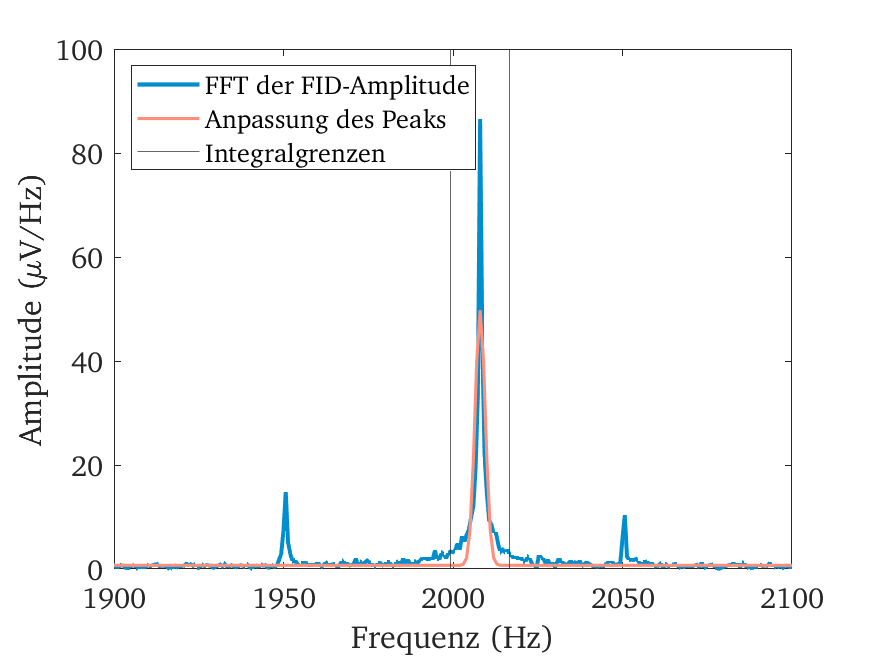
\includegraphics[width=\textwidth]{Bilddateien/7/Part7_Fig_2.png}
        \caption{Fouriertransformation des FID der Wasserflasche aus Abb. \ref{fig:FID_Optimised}.}
        \label{fig:FID_Optimised_FFT}
    \end{figure}